\documentclass[11pt,oneside]{book}
\usepackage{underscore}
\usepackage[margin=1in]{geometry}
\usepackage{xcolor}
\usepackage[hidelinks]{hyperref}
\usepackage{graphicx}
\usepackage{accsupp}
\ifdefined\darkmode\pagecolor[HTML]{091117}\color[HTML]{F0EDE4}\def\viewtheme{dark}\else\def\viewtheme{light}\fi
\title{GoServer\\[0.5em]\large N-player Go in the spirit of KGS}
\author{Project team}
\date{\today}
\begin{document}
\frontmatter
\maketitle
\tableofcontents
\mainmatter

% ---------------------------------------------------------------------------
\chapter{What GoServer is}
GoServer is a local, in-memory online Go service for \emph{multiplayer} Go:
two to eight players on one board, each with a colour, taking turns in order.
KGS inspires the navigation (rooms, challenges, chat) but there is no
compatibility with KGS accounts, protocols or clients. The rules engine is a
port of the stakeholder's single-page N-Player Go Lab, whose JavaScript
(\path{source/cmd/demo/static/engine.js}) remains the reference.

A visitor picks a display name, enters a room, talks in room chat and opens or
creates a challenge. The creator chooses the board and clocks, decides seat by
seat whether a person or a bot plays and who is on which team, and starts the
game. Empty seats become bots that search with Monte Carlo tree search on the
server. During play a person can hand their seat to a bot (autopilot) and take
it back, and teams can merge when everyone on both teams agrees. Every viewer
can step through the game's history and see each bot move's search; watchers
can branch and run their own searches, which never reach the server.

The record of the project is this book together with
\path{spec/Requirements.lean}, \path{spec/Requirements.proto},
\path{spec/Implementation.lean} and the source in \path{source/}. Review and
acceptance happen in git; chat histories are disposable.

\section{Running it}
From the project root:
\begin{itemize}
  \item \texttt{make run} builds and serves the app on \texttt{127.0.0.1:8081}
  (\texttt{make run PORT=8090} picks another port; LeanFM's own 8080 is never
  used); \texttt{make stop} stops only the process it started.
  \item \texttt{make spec-check} runs LeanFM's canonical check on the three
  specification files and regenerates \path{spec/tasks.json}.
  \item \texttt{make views} derives the task figures of Appendix~\ref{ch:catalog}
  from that catalog.
  \item \texttt{make app-check} builds and runs \texttt{go test -race}.
  \item \texttt{make browser-check} drives a real headless Chrome through two
  users' room, challenge and chat flow; \texttt{make tour} replays the usage
  scenarios of Chapter~\ref{ch:usage} and refreshes their screenshots.
  \item \texttt{make book} rebuilds this book in light and dark copies.
\end{itemize}
All state lives in memory and resets on restart. Building needs Go and Node.js
with npm: the browser app is a React project in \path{source/web} that
\texttt{make run} builds first (the first build runs \texttt{npm ci}).

% ---------------------------------------------------------------------------
\chapter{Rooms, challenges and chat}
\section{Navigation}
After choosing a name a person is in the lobby. Every room they have open is a
tab along the top, and a final \emph{+ Rooms} tab lists all rooms and creates
new ones. Inside a room, the first tab is its Lobby: the room conversation, its
challenges and the form for a new challenge. Opening a challenge adds a tab for
that game, so several games can be open at once, in one room or in several. A
game's tab shows its seats, its board once started, and its own chat. Tabs stay
alive in the background, keeping each game's variations and analysis; a room tab
counts unread messages, and a game tab is marked when a move or a merge answer
is waiting for the viewer. Open tabs come back after reloading the page. Each tab
shows only results requested for its own room or game, so a slow response can
never appear in another tab.
Room chat and game chat are separate conversations: nothing posted in one is
copied to the other, and only members of a room or game receive its chat.
Watching or joining a game enters its chat; neither grants any move authority.

\section{Identity}
The server issues the session; creator and sender are always derived from it,
never taken from request fields. A name is free until its holder claims it with
a password (chapter~\ref{ch:claims}); an unclaimed display name identifies a
person for the life of the server, as before.
Sessions live in memory, so restarting the server forgets them; a page
that still holds a forgotten session returns to the name form, prefilled with
the previous name, and says why.

\section{Bounds}
Names are 1--128 Unicode characters, trimmed; room names are unique and
case-sensitive and are never interpreted as paths or markup. Chat bodies are
1--4000 characters, and each room or game keeps its latest 100 entries. There
are at most 16 rooms including the lobby and 64 challenges in total. Each
session has a finite budget of admitted mutations; once it is spent, new
mutations are rejected while already accepted results stay replayable, so a
retried request never applies twice.

\section{Correlation and replay}
Every request carries a request ID unique per session and task, and receives
exactly one result: its success message or \texttt{RequestRejected}, with the
same ID. A duplicate mutation returns the earlier result; reusing an ID with a
different body is rejected. A rejected or overloaded request changes nothing
and discloses no other person's identity or session.

% ---------------------------------------------------------------------------
\chapter{N-player Go rules}
\section{Board, turns and captures}
The board has 5, 7, 9, 11, 13 or 19 lines and is bounded by a Wall. Seats move
in order. After a stone is placed, every adjacent group of \emph{another}
colour left without liberties is removed first. Only if nothing was captured
and the placed stone's own group has no liberties is the move a suicide, and
then that whole group is removed. Suicide is legal: in multiplayer Go a player
may sacrifice a group to help an ally make eyes.

\section{Losses, bowls and score}
A removed stone counts against its \emph{owner}, not for the capturer: it goes
to the owner's losses, and the bowl records which seat captured it (suicide is
recorded against the mover). Territory is an empty region bordered only by one
colour's stones and the Wall. A seat's score is its territory minus its losses;
a team's score is the sum of its members' territory minus the sum of their
losses,
\[
  S_T = \sum_{p\in T} A_p - \sum_{p\in T} G_p .
\]
The winners are the team or teams with the highest score among teams that still
have a member who has not resigned.

\section{Ko and repetition}
The ko rule is a challenge parameter: \emph{Auto} (the default: on for two
players, off for three or more), \emph{Off}, or \emph{On}. When on it is simple
ko plus \emph{situational} superko: a stone may not recreate an earlier board
with the same seat to move. The Lab calls this ``positional superko'', but its
comparison includes the player to move, so situational is the accurate name.
A Zobrist hash only indexes candidates; equality is decided on the exact board
and seat, so a hash collision can never reject a legal move. Passes, timeouts
and resignations are never rejected for repeating a position.

\section{Clocks and ending}
A person's turn has a deadline (5 seconds to 64 minutes, default one minute); a
bot's search has its own budget (0.25 to 16 seconds, default 1 second). An
unanswered turn becomes a \emph{timeout}: it passes the turn but neither ends
nor resets a round of passes. A move arriving after its deadline is rejected
and the timeout wins. The game ends when every remaining seat has passed since
the last stone, after one full round of timeouts (scored as it stands), or at
\(3N^2\) moves on an \(N\times N\) board. A resigned seat passes automatically
and cannot win. The final scores and winners are announced in game chat.

\section{Challenge parameters}
Board size (default 11), seats 2--8 (default 4), the two clocks, the ko rule,
and the bot settings of the Lab: exploration constant 0.5, 0.7 (default), 1.0
or 1.4; reward \emph{margin} (a soft margin against the best rival, the
default), \emph{win} or \emph{rank}; and margin softness 2, 4 (default) or 8
points. Zero or empty means the default; anything out of range is rejected.

% ---------------------------------------------------------------------------
\chapter{Seats, bots and teams}
\section{Seat plan}
Before the start the creator plans each seat as \emph{bot} or \emph{open} and
gives it a team number from 1 to the seat count; by default each seat is its
own team. People in the room take open seats (one seat per person per game) or
leave them. A seat planned as a bot cannot be taken, and a seat a person holds
cannot be turned into a bot seat until that person leaves. Only the creator
starts the game; every seat still without a person becomes a bot named
\texttt{bot-}\emph{seat}. Seats never change after the start.

\section{Bots}
Bots run Monte Carlo tree search on the server, for their team's combined
score. A bot turn is dispatched to a bounded pool of search workers (at most
\(\min(8, \textit{CPUs}/2)\) at once), each with a time budget and a 200,000-node
cap, and the search never holds the game lock. A result is applied only to the
game, seat and turn revision it was dispatched for, and only before that turn's
deadline; a late result is discarded (Figure~\ref{fig:bot_turn}). No client can
submit a bot's move, and a bot never moves for a person's seat. Each bot move
publishes its search: playouts, time, the top candidates with visit counts, the
mover's expected reward, and every seat's projected final score and outlook.

\section{Autopilot}
A seated person may switch autopilot on, letting a server bot play their seat
with the bot clock and published search, and switch it off at any time. The
seat, team and name stay theirs. Switching off during their own turn discards
the pending bot result and gives them the rest of the human deadline, measured
from the start of the turn.

\section{Team merges}
During play a seated person may propose merging their team with another team
that also has a seated person (nobody could consent for an all-bot team). The
merge happens once every person seated in either team accepts; it takes the
smaller team number and is permanent. Any decline, any change to either team,
or the game finishing withdraws the proposal; there is at most one pending
proposal per pair of teams. Bots of the merged team then search for its
combined score (Figure~\ref{fig:team_merge}).

% ---------------------------------------------------------------------------
\chapter{Claimed names and ranking}
\label{ch:claims}
\section{Claiming a name}
Anyone can enter any free name. To keep it, the person signed in under that
name opens the Ranking tab and sets a password (8 to 128 characters, typed
twice). From then on the server gives a session for the name only with that
password; signing in with it ends any older session for the name, and the person
keeps their rooms, games and seats, because those belong to the name. Claims
ignore letter case and surrounding spaces, so \texttt{Alice} and
\texttt{alice} are one name, and a claim is refused while someone else is
signed in under a case variant. Names beginning \texttt{bot-} belong to bots
and nobody can sign in with one.

The server stores a salted PBKDF2-SHA256 hash (600{,}000 rounds), never the
password. After five wrong passwords in a row for one name, each further
attempt waits twice as long as the last (2 seconds, then 4, up to 15 minutes),
and only one attempt per name is checked at a time; at most two hashes are
computed at once. There is no password reset: a forgotten password means a new
name.

\section{Which games count}
A finished game is \emph{rated} when seats on at least two different teams are
held by different rated players. A bot is rated by its search settings (time,
exploration, reward), so a 4-second bot and a 1-second bot are different
players and beating the stronger one counts for more. A person is rated only if
their exact name was claimed before the game started and their seat never
switched to autopilot. Other seats still play; they just do not feed the
ranking. Games before a claim never count, because anyone could have used the
name then.

\section{The rating}
Teams are placed by whether they still have a member who has not resigned, then
by team score; equal teams share a place. Every two rated seats on different
teams make one comparison: a win and a loss, or half of each when the teams
tie. Each pair of teams carries a total weight of one, shared among their rated
members, so a team of three does not outvote a lone player.

The ratings are the Bradley--Terry maximum-likelihood fit over all comparisons,
on the Elo scale (400 points per factor of ten in strength). Every player also
gets one win and one loss against a fixed 1500 anchor, which keeps ratings
finite and holds players with few games near 1500. The fit uses every recorded
game at once, so the ranking never depends on the order in which games finished,
and recomputing it from the file always gives the same numbers: the weights are
exact integers, so even the floating-point sums do not depend on order. Some
values from the tests:
\begin{itemize}
  \item One game, A beats B: A 1592, B 1408 (checked by hand).
  \item One four-player game in places 1 to 4: 1713, 1566, 1434, 1287.
  \item A team of A and B beats C: A and B 1551 each, C 1396.
\end{itemize}
The Ranking tab lists claimed names and bots by rating, with each one's rated
games and first places; it refreshes every ten seconds.

\section{What survives a restart}
Claims and rated results are appended to \path{data/goserver.jsonl} in the
project folder (\texttt{GOSERVER\_DATA\_DIR} overrides it). Each record is one
line, flushed to disk before the claim is acknowledged. On start the file is
replayed: a line cut off by a crash is dropped, and any other damaged line stops
the start with its line number rather than silently losing history. The folder
is private to the user (mode 0700, file 0600), symlinks are refused, and no web
route reads it. Up to 1000 claims and 100{,}000 rated games are kept; beyond
that a game says in its chat that it was not added. Rooms, games, chat and
sessions still reset on restart.

\chapter{What every viewer sees}
The browser reproduces the Lab against server state:
\begin{itemize}
  \item the board with Wall coordinates, territory squares, the last-move
  marker, ghost markers for next moves and a search heat overlay;
  \item a translucent stone in the mover's colour under the pointer wherever a
  click would place a stone (the viewer's own live turn, or a variation where
  analysis is open to them); over an occupied or forbidden point, or out of
  turn, there is no preview and the pointer shows that a click would be refused;
  \item player colours drawn as stones on a small wood tile, so a black stone
  never reads as a hollow white ring on the dark page;
  \item an always-visible play bar (whose turn it is, the clock, Pass, Resign,
  autopilot) above tabs for Scores, Search, Seats, Chat and GIF; the Chat tab
  counts unread messages and the Seats tab flags a merge awaiting the viewer's
  answer;
  \item navigation with Home, Back, Forward, End and previous/next variation,
  by buttons and by the arrow, Home and End keys; a variation tree and next-move
  chips;
  \item a \emph{Search at this position} panel listing candidate moves with
  visit share and reward, from the bot's published search or the viewer's own;
  \item per seat: Territory, Bowl, Score, Proj.\ (projected final score) and
  Outlook (expected reward), and team totals;
  \item a clickable projected-score timeline along the viewed line;
  \item pending merge proposals with who has accepted and who must still answer;
  \item GIF export of the viewed line, and stone, capture and last-ten-seconds
  sounds with a toggle;
  \item live following while at the latest move, otherwise a notice that new
  moves arrived.
\end{itemize}
Variations and local searches run in the viewer's browser with the Lab engine
on a copy of the position. They are never sent to the server, never change the
game, and vanish when the page closes. Watchers may branch and search at any
time; a person seated in a game in play may browse the actual moves, and may
branch and search once the game has finished. That last rule is a fairness
convention of the provided browser, not a security boundary: a public position
can always be copied into another tool. The page is dark-only, and its text
is always light on a dark background: highlighted buttons and tags use yellow
text and a yellow border on a dark fill, never dark text on yellow, so a
browser's dark-mode extension cannot turn them into white on yellow.

% ---------------------------------------------------------------------------
\chapter{Requirements}
\section{Shape}
\path{spec/Requirements.lean} declares two actors that people see,
\texttt{Person} and \texttt{Server}, and a third, \texttt{Bot}: the bounded pool
of server search workers. Every operation is a task whose grammar is a request
followed by its correlated success or \texttt{RequestRejected}. Five tasks are
composed: \texttt{bot\_turn}, \texttt{turn} (a person's move, a bot turn, a
timeout or an automatic pass), \texttt{team\_merge}, and
\texttt{game\_lifecycle}: create, then any number of seat, join, chat and state
operations, then start, then turns, autopilot switches, merges, chats and state
reads, until \texttt{GameFinished} (Figure~\ref{fig:game_lifecycle}).
Server-originated events (\texttt{BotMovePlayed}, \texttt{TurnTimedOut},
\texttt{AutoPassed}, \texttt{TeamsMerged}, \texttt{MergeWithdrawn},
\texttt{GameFinished}) reach game members as entries of \texttt{GameState}, and
\texttt{GetGameState} takes \texttt{since\_move} so a viewer fetches only new
move records. \path{spec/Requirements.proto} declares the same messages.

\section{Positive invariants}
Every room, chat, board, clock, score and team a viewer sees comes from one
server-authoritative transition in a scope the viewer is authorized for. Every
turn ends exactly once (\(AG(\textit{to\_move} \Rightarrow AF\,\textit{moved})\)),
and every started game finishes (\(AG(\textit{playing} \Rightarrow AF\,\textit{finished})\)).

\section{Negative requirements and their controls}
Each \emph{never} obligation of the specification is held by a control and a
test; \path{source/traceability.json} lists them in full.
\begin{itemize}
  \item \textbf{A move for another seat, out of turn, or for an autopilot seat}:
  seat-to-move identity check under the game lock
  (\texttt{TestMovesAreAuthorizedOrderedAndRuleChecked}).
  \item \textbf{Two transitions for one turn} (move, bot result, timeout,
  auto-pass): a turn sequence number under the lock and the replay cache
  (\texttt{TestTurnsNeverEndTwice}).
  \item \textbf{A move accepted after its deadline}: the deadline is rechecked
  on arrival and the timeout applied first (\texttt{TestLateMoveLosesToTheDeadline}).
  \item \textbf{A stale or misdirected bot result}: results bound to game, seat
  and turn revision (\texttt{TestBotNeverMovesForAHuman},
  \texttt{TestAllBotGamePlaysToTheEnd}).
  \item \textbf{A legal move rejected by a hash collision}: exact situation
  compared behind the Zobrist key (\texttt{TestSituationalSuperkoUsesExactPositions}).
  \item \textbf{Unbounded bot work}: search outside the lock, time budget, node
  cap, bounded slots (race-enabled \texttt{TestAllBotGamePlaysToTheEnd}).
  \item \textbf{A merge without consent}: per-person acceptance sets and
  withdrawal on any team change (\texttt{TestMergesNeedEveryPersonsConsent},
  \texttt{TestTeamChangeAndFinishWithdrawProposals}).
  \item \textbf{Seat or plan changes by the wrong person or after the start}:
  creator and status checks (\texttt{TestSeatPlanIsTheCreatorsBeforeStart},
  \texttt{TestSeatsStartAndBotsFillEmptySeats}).
  \item \textbf{Crossing a room or game boundary}: membership checks on every
  read and write (\texttt{TestNamedChallengesAndChatHistoryStayInScope}).
  \item \textbf{Executable user text, fabricated destinations, stale responses
  replacing another scope, exposed tokens}: text-only DOM rendering,
  selection-generation guards, strict bounded JSON, Host and Origin checks
  (\texttt{TestMethodOriginHostAndBodyRejections}, \texttt{browser\_check.py}).
  \item \textbf{A pointer preview that promises a refused move, or talks to
  the server}: the preview is gated by the same predicates as a click and drawn
  only on the canvas (\texttt{TestViewerTabsAndPointerPreview}; the usage tour
  hovers an empty and an occupied point in Chrome).
  \item \textbf{A claimed name used without its password}, including case
  variants and bot names: claim lookup by lower-cased name, constant-time hash
  comparison, the per-name doubling delay (\texttt{TestClaimNameAndSignIn},
  \texttt{TestWrongPasswordsAreThrottled}, \texttt{TestClaimSignInAndRankingOverHTTP},
  \texttt{browser\_check.py}).
  \item \textbf{A password kept or shown}: only a salted hash is stored; the
  claim never enters the replay cache; responses, the page, its storage and the
  data file are checked for it (\texttt{TestClaimNameAndSignIn},
  \texttt{TestDataFileIsDurableAndRefusesDamage}, \texttt{browser\_check.py});
  PBKDF2 is checked against RFC~7914 (\texttt{TestPBKDF2MatchesRFC7914Vector}).
  \item \textbf{A rating from a game that should not count}, or a game counted
  twice or depending on order: claim time against game start, the autopilot
  flag, random result identities, exact integer weights
  (\texttt{TestFinishedGamesFeedTheRanking}, \texttt{TestFitMatchesIndependentNewtonFit},
  checked against an independent Newton's-method fit).
  \item \textbf{A claim acknowledged before it is on disk, or a damaged or
  escaping data file}: write and flush before acknowledging, torn-tail
  truncation, refusal of other damage and of symlinks
  (\texttt{TestClaimIsNotAcknowledgedUntilDurable},
  \texttt{TestDataFileIsDurableAndRefusesDamage}, \texttt{TestDataPathRefusesSymlinksAndEscapes}).
  \item \textbf{A game that never ends}: passes, the timeout round and the
  \(3N^2\) cap (\texttt{TestPassesEndTheGame},
  \texttt{TestDeadlineTimesOutAndAbandonmentEnds}).
\end{itemize}

\section{Derived outputs}
Besides the task views, the specification asks for two outputs: the
projected-score timeline (per seat, against move number, from bot searches and
the viewer's local searches), and the game result (team scores and winners).

% ---------------------------------------------------------------------------
\chapter{Implementation}
\path{spec/Implementation.lean} maps the specification onto Go. The server
(\path{source/server.go}, \path{source/game.go}) holds rooms, games and chat in
memory behind per-game locks; \path{source/engine.go} ports the Lab's rules and
max-n Monte Carlo search, extended to return the Lab's search summary;
\path{source/bot.go} is the bounded worker pool that realizes the \texttt{Bot}
actor; \path{source/channel.go} is the bounded queue whose full sends block
until space frees, as the requirements' channel semantics demand.

The browser app is React and TypeScript in \path{source/web}, so its parts can be
rearranged as components: \path{App.tsx} holds the room tabs, \path{Room.tsx} a
room's Lobby and game tabs, \path{Game.tsx} one game (board column, play bar and
side tabs), \path{Board.tsx} and \path{Panels.tsx} the pieces, and
\path{game/game.ts} the controller for one open game (the Lab game tree, server
sync, local search). Vite builds it into \path{source/cmd/demo/static/app/},
which the Go demo embeds. The Lab rules engine, \path{static/engine.js}, loads
first as a plain script and stays the single rules reference for the browser
and for \path{source/engine.go}. The demo serves the engine and search worker as
same-origin files, so viewers can branch and search locally under a content
security policy that adds only same-origin workers and
\texttt{blob:}/\texttt{data:} images for GIF preview.

The HTTP demo in \path{source/cmd/demo/} carries the protobuf-shaped messages
as bounded JSON. It is an inspection harness for the server core, not evidence
of protobuf byte conformance and not a production account system.

\section{Evidence}
\begin{itemize}
  \item \path{reports/specification-check/validation.json}: the canonical check
  of the three specification files, with their hashes.
  \item \texttt{go test -race ./...} in \path{source/}: unit, concurrency and
  negative tests named above.
  \item \path{reports/browser/}: the two-user Chrome check and its screenshot.
  \item \path{book/assets/tour/manifest.json}: the scripted usage tour, with
  image hashes, source hashes and browser version.
\end{itemize}
A passing check establishes elaboration, protobuf agreement, structural
completeness and the provenance of the figures. It does not prove that the
running server satisfies the temporal, isolation, concurrency or resource
obligations; those rest on the controls and tests above.

% ---------------------------------------------------------------------------
\IfFileExists{tour.tex}{% Generated by source/book_tour.py; do not edit by hand.
\chapter{Usage scenarios}
\label{ch:usage}
These screenshots come from the running application, driven by a script that plays the parts of three people: alice creates the challenge, bob joins her, and carol watches. \texttt{make tour} in the project root reproduces them; \path{book/assets/tour/manifest.json} records each step, viewer, image hash, source hashes and browser version. Bot moves come from a time-limited search, so the stones differ between runs while the steps do not.

\section{Welcome}
A visitor chooses a local display name. Nothing else is needed for the local preview.

\begin{figure}[ht]
\centering
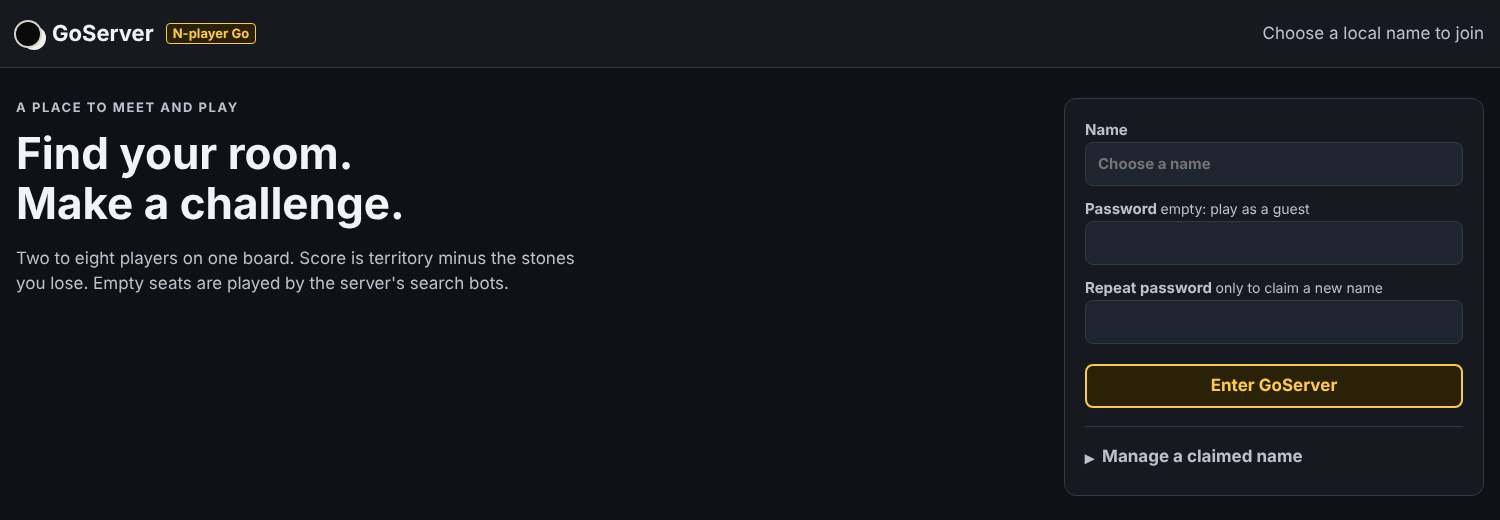
\includegraphics[width=\textwidth]{assets/tour/01-welcome.png}
\caption{Welcome, seen by alice. Steps: open the app.}
\end{figure}
\clearpage

\section{Creating a challenge}
Alice is in the lobby and fills in a challenge: a 9$\times$9 board, three players, and a byo-yomi clock of one minute of main time and then three periods of ten seconds, the same for people and bots. The ko rule stays on Auto, which is off for three players.

\begin{figure}[ht]
\centering
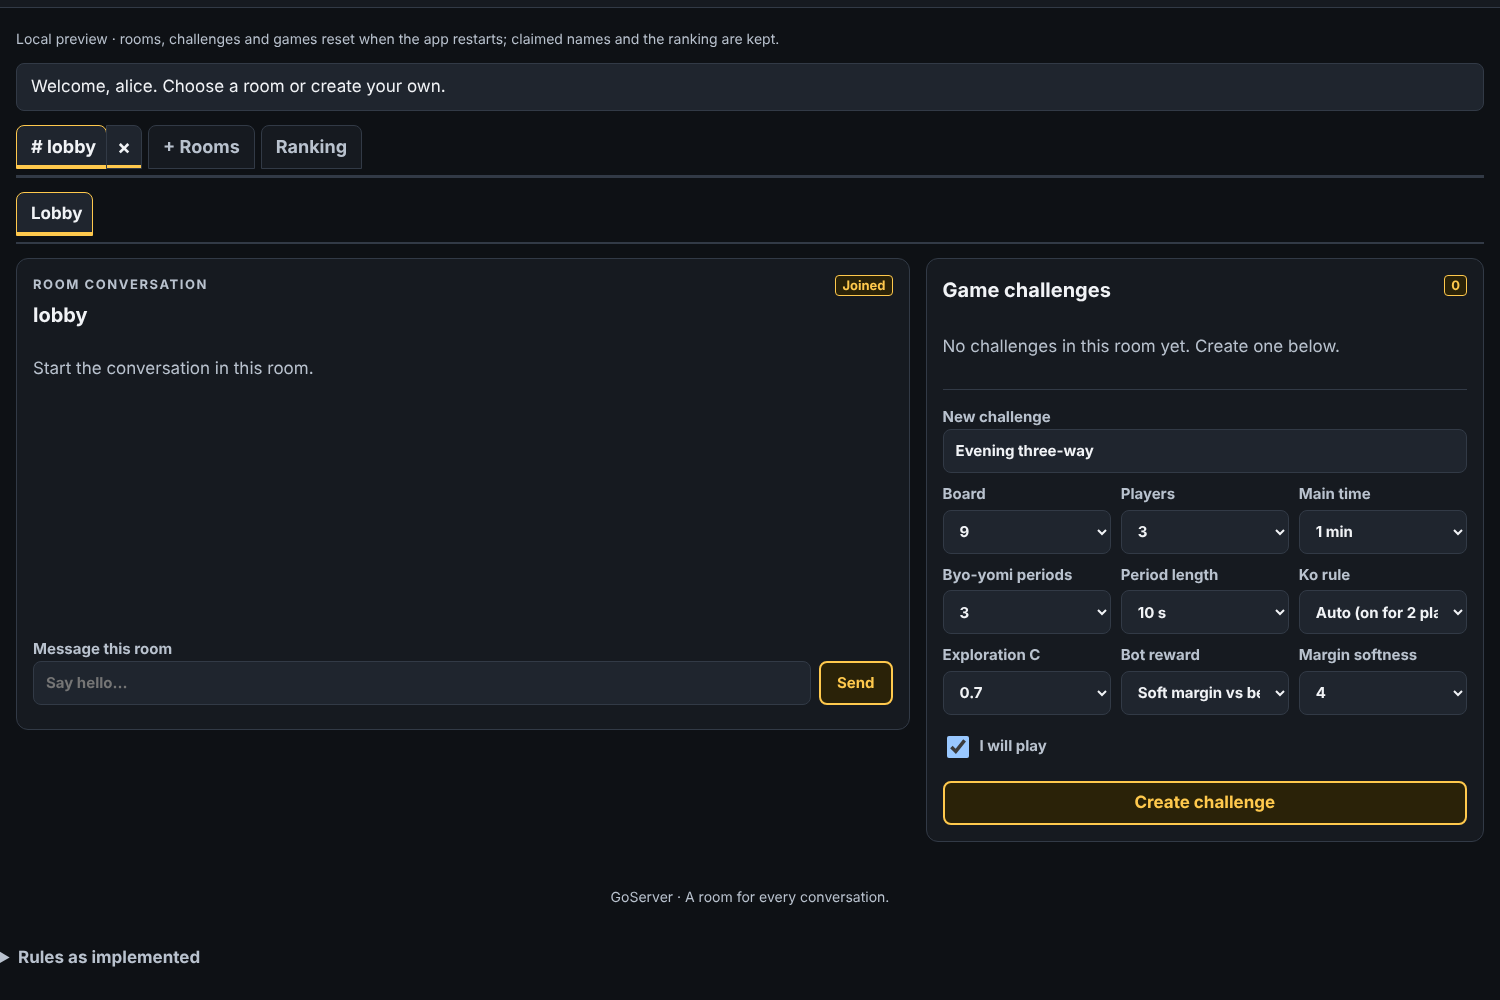
\includegraphics[width=\textwidth]{assets/tour/02-create-challenge.png}
\caption{Creating a challenge, seen by alice. Steps: sign in as alice; fill in the New challenge form.}
\end{figure}
\clearpage

\section{Planning seats}
Before the start the creator decides, seat by seat, whether a person or a bot plays and which team the seat is on. Alice took seat 1, bob sat in seat 2, and alice marked seat 3 as a bot.

\begin{figure}[ht]
\centering
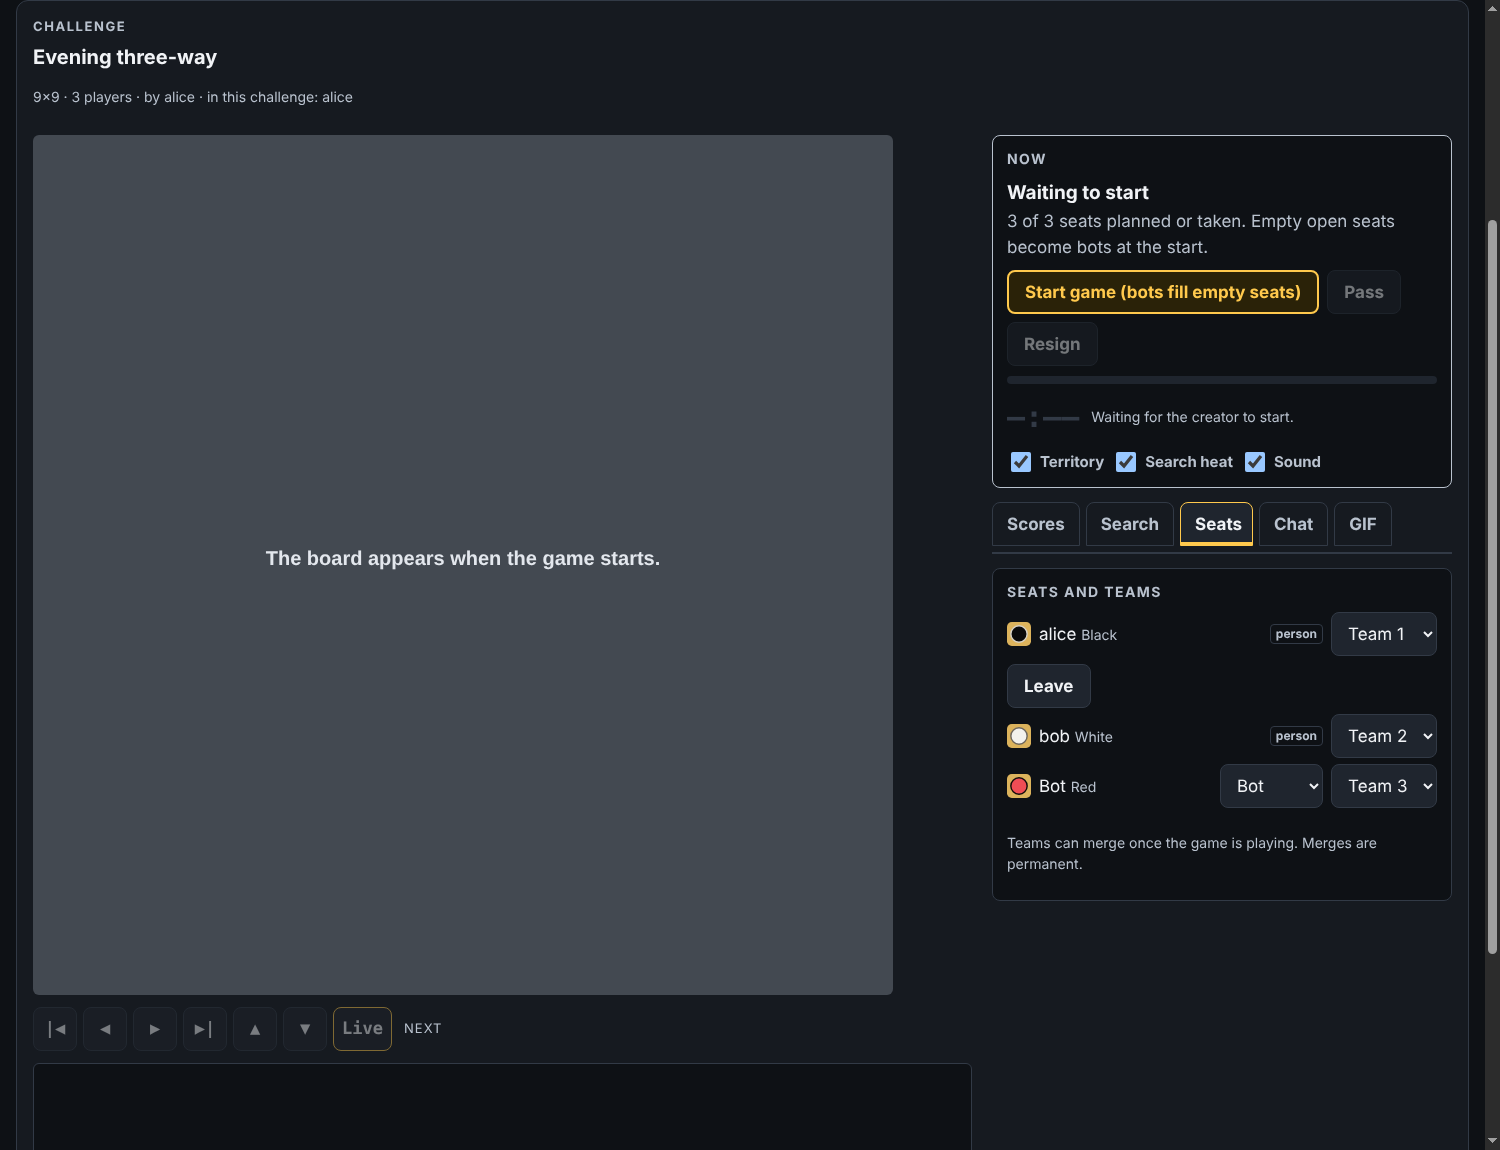
\includegraphics[width=\textwidth]{assets/tour/03-seat-plan.png}
\caption{Planning seats, seen by alice. Steps: alice: create the challenge (seated automatically); alice: set seat 3 to Bot; bob: open the challenge, Sit here.}
\end{figure}
\clearpage

\section{Aiming a stone}
On her turn alice moves the pointer over the board: a translucent stone in her colour shows exactly where a click will play. Over an occupied point, a point the ko rule forbids, or when it is not her turn, there is no preview and the pointer shows that a click would be refused. Above the tabs, the play bar keeps whose turn it is and the clock in view.

\begin{figure}[ht]
\centering
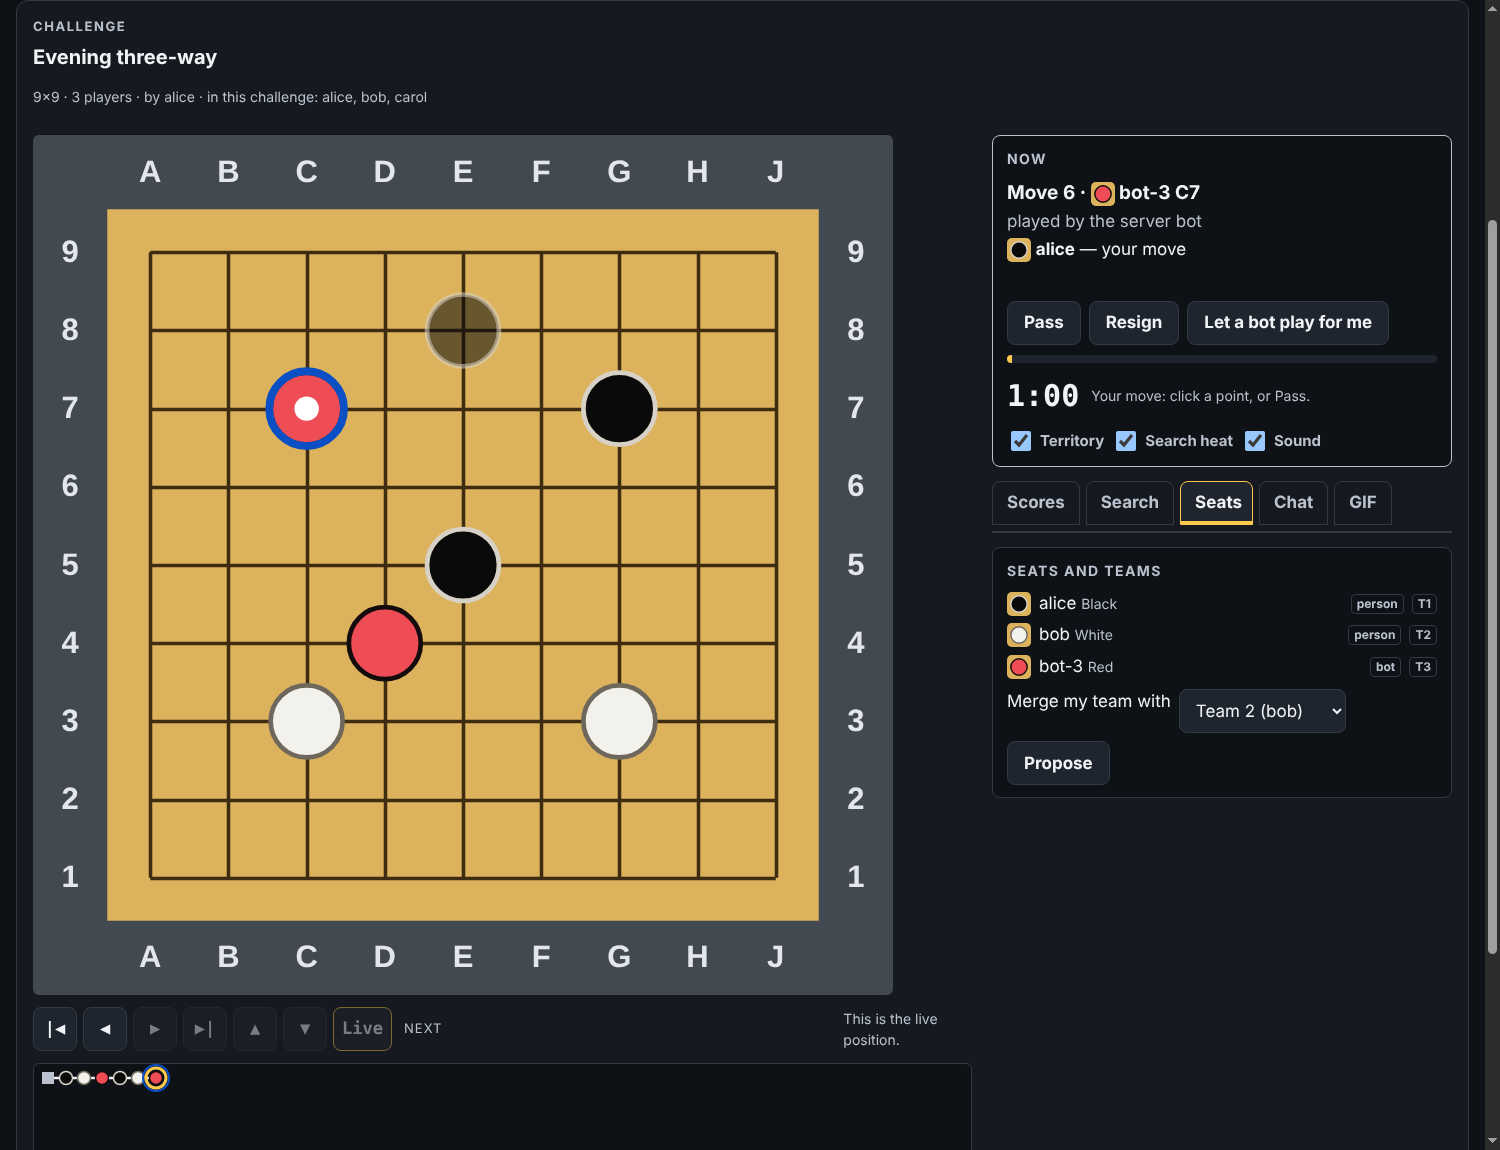
\includegraphics[width=\textwidth]{assets/tour/04a-aim.png}
\caption{Aiming a stone, seen by alice. Steps: alice: move the pointer over an empty point on her turn.}
\end{figure}
\clearpage

\section{Reading the bot's search}
Alice steps back one move, to the position where the bot searched for its last move. The panel lists the moves that search weighed, with visit share and expected reward; the blue discs on the board are the same search as a heat map. Proj. and Outlook give every seat's projected final score and expected reward, and the timeline under them plots the projections move by move.

\begin{figure}[ht]
\centering
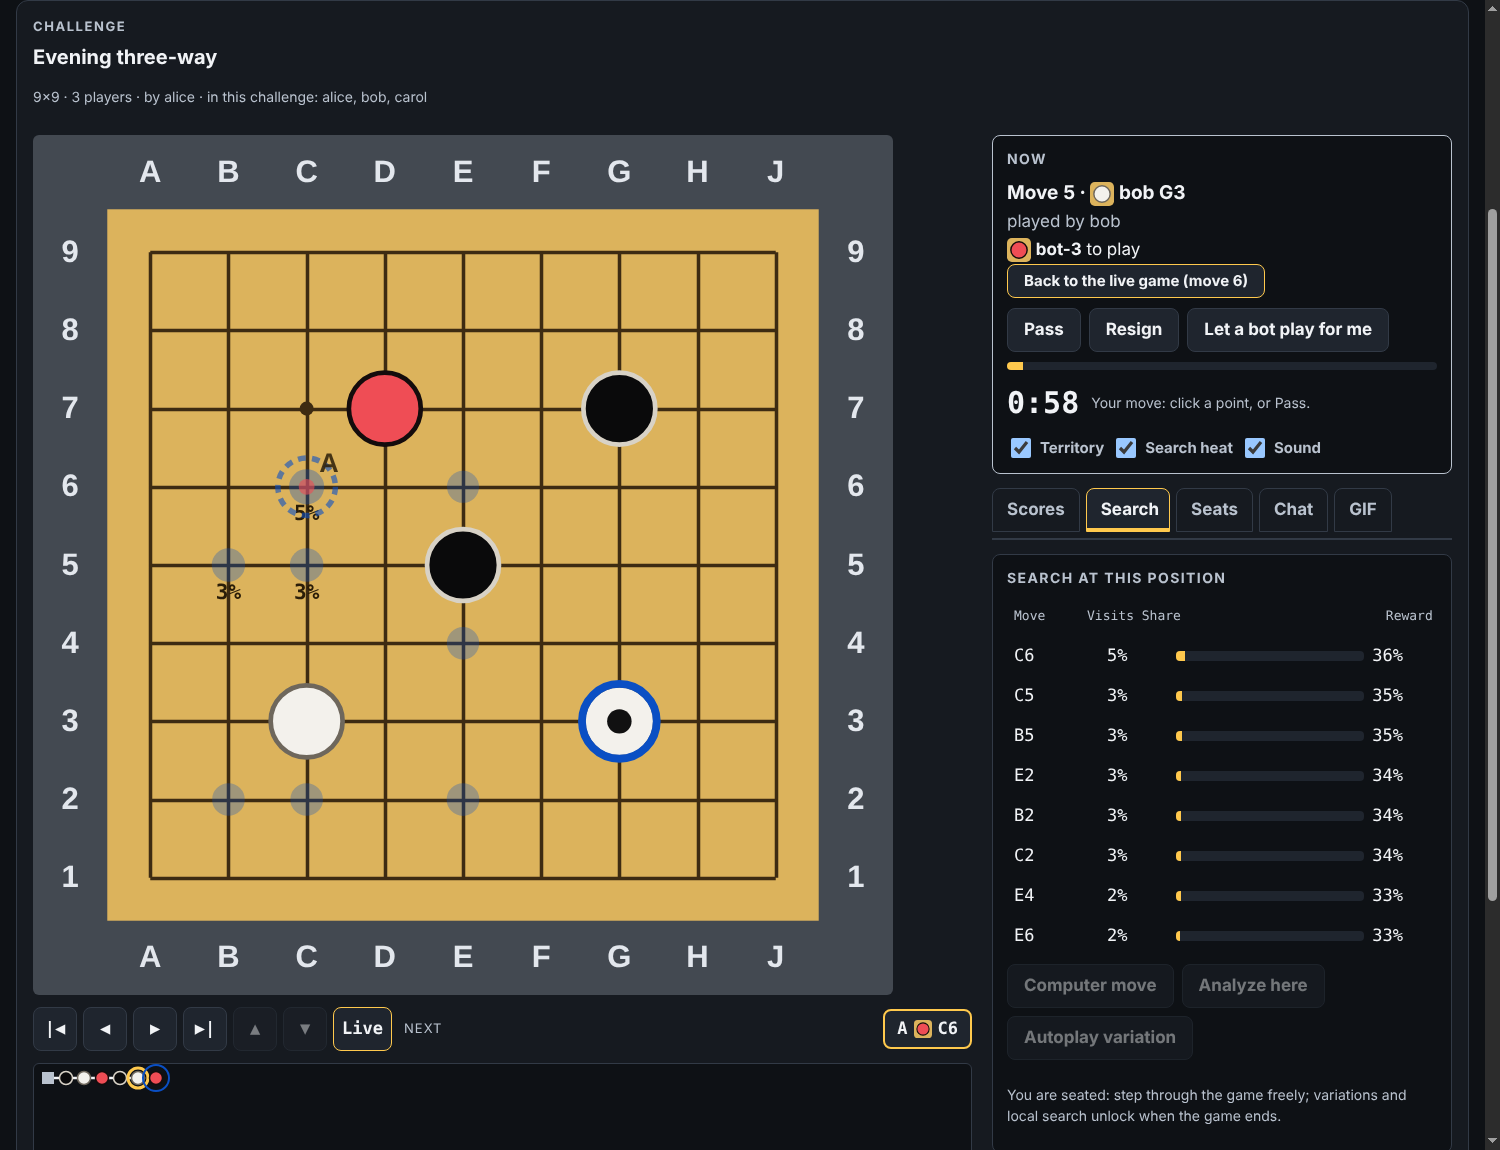
\includegraphics[width=\textwidth]{assets/tour/04-bot-search.png}
\caption{Reading the bot's search, seen by alice. Steps: alice and bob alternate stones by clicking the board; the bot answers each round; alice: Back one move.}
\end{figure}
\clearpage

\section{A watcher explores a variation}
Carol is watching, not playing. She steps back to move 3, tries a different stone (the gold ring marks a variation), and asks for a local search. The analysis runs in her browser only: the dashed branch in the tree never reaches the server, and the live game continues.

\begin{figure}[ht]
\centering
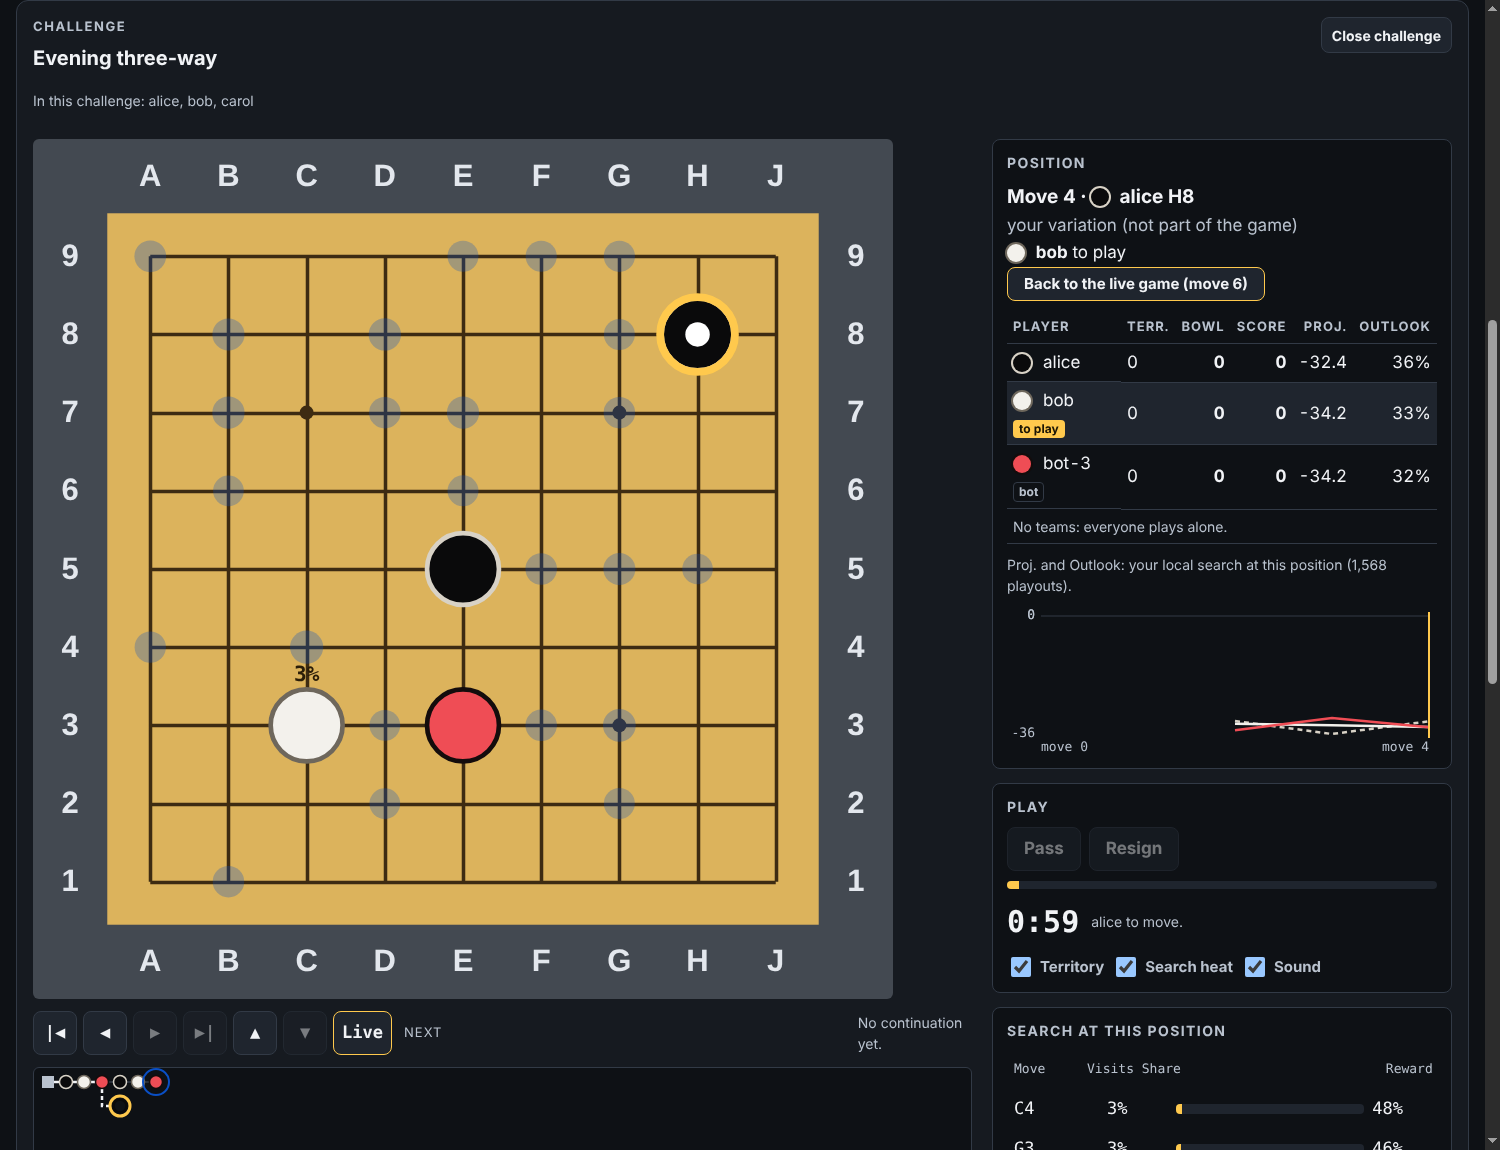
\includegraphics[width=\textwidth]{assets/tour/05-watcher-variation.png}
\caption{A watcher explores a variation, seen by carol. Steps: carol: open the challenge as a watcher; carol: Home, then Forward three times; carol: click an empty point; carol: Analyze here.}
\end{figure}
\clearpage

\section{Proposing a team merge}
During play bob proposes merging his team with alice's. The Seats tab flags a proposal waiting for her answer; there the proposal shows who has accepted and who is still to answer; it takes effect only when every person on both teams accepts, and it is permanent.

\begin{figure}[ht]
\centering
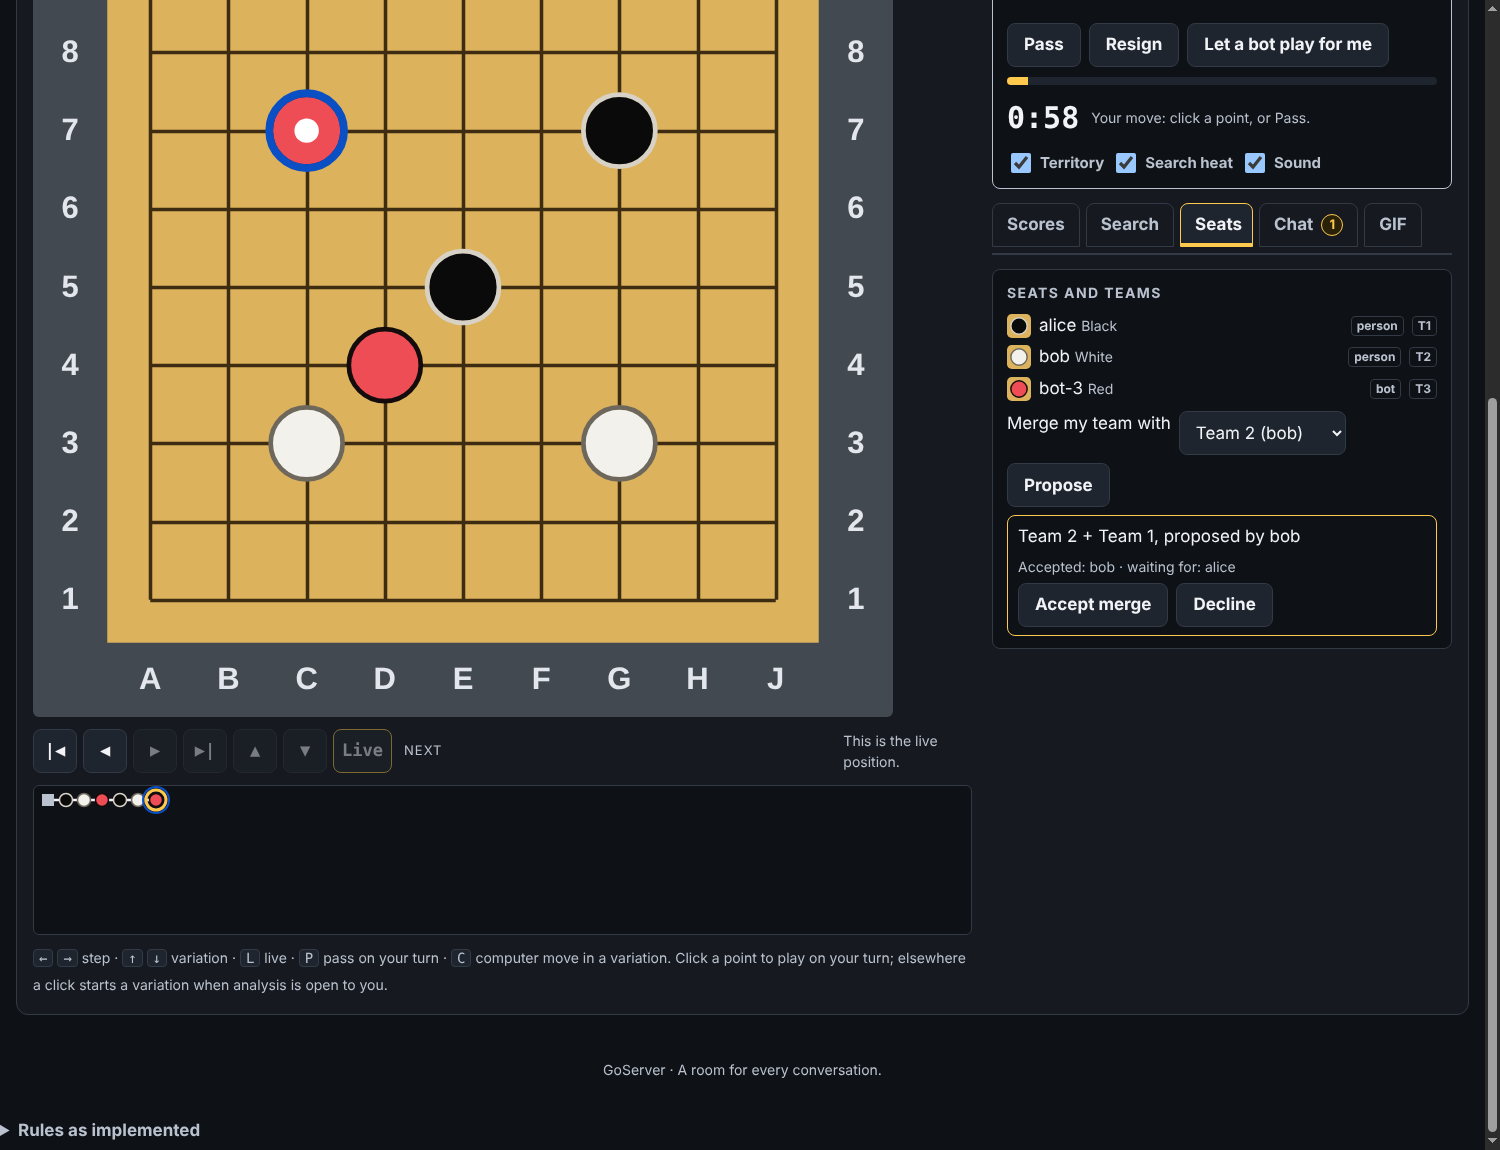
\includegraphics[width=\textwidth]{assets/tour/06-merge-proposal.png}
\caption{Proposing a team merge, seen by alice. Steps: bob: Merge my team with Team 1, Propose.}
\end{figure}
\clearpage

\section{Playing as a team, on autopilot}
After the merge the score table shows alice and bob as team 1 with a combined total. Alice then lets a bot play her seat; the seat, team and name stay hers, and the bot's move publishes its search like any other bot move. She can take the seat back at any time.

\begin{figure}[ht]
\centering
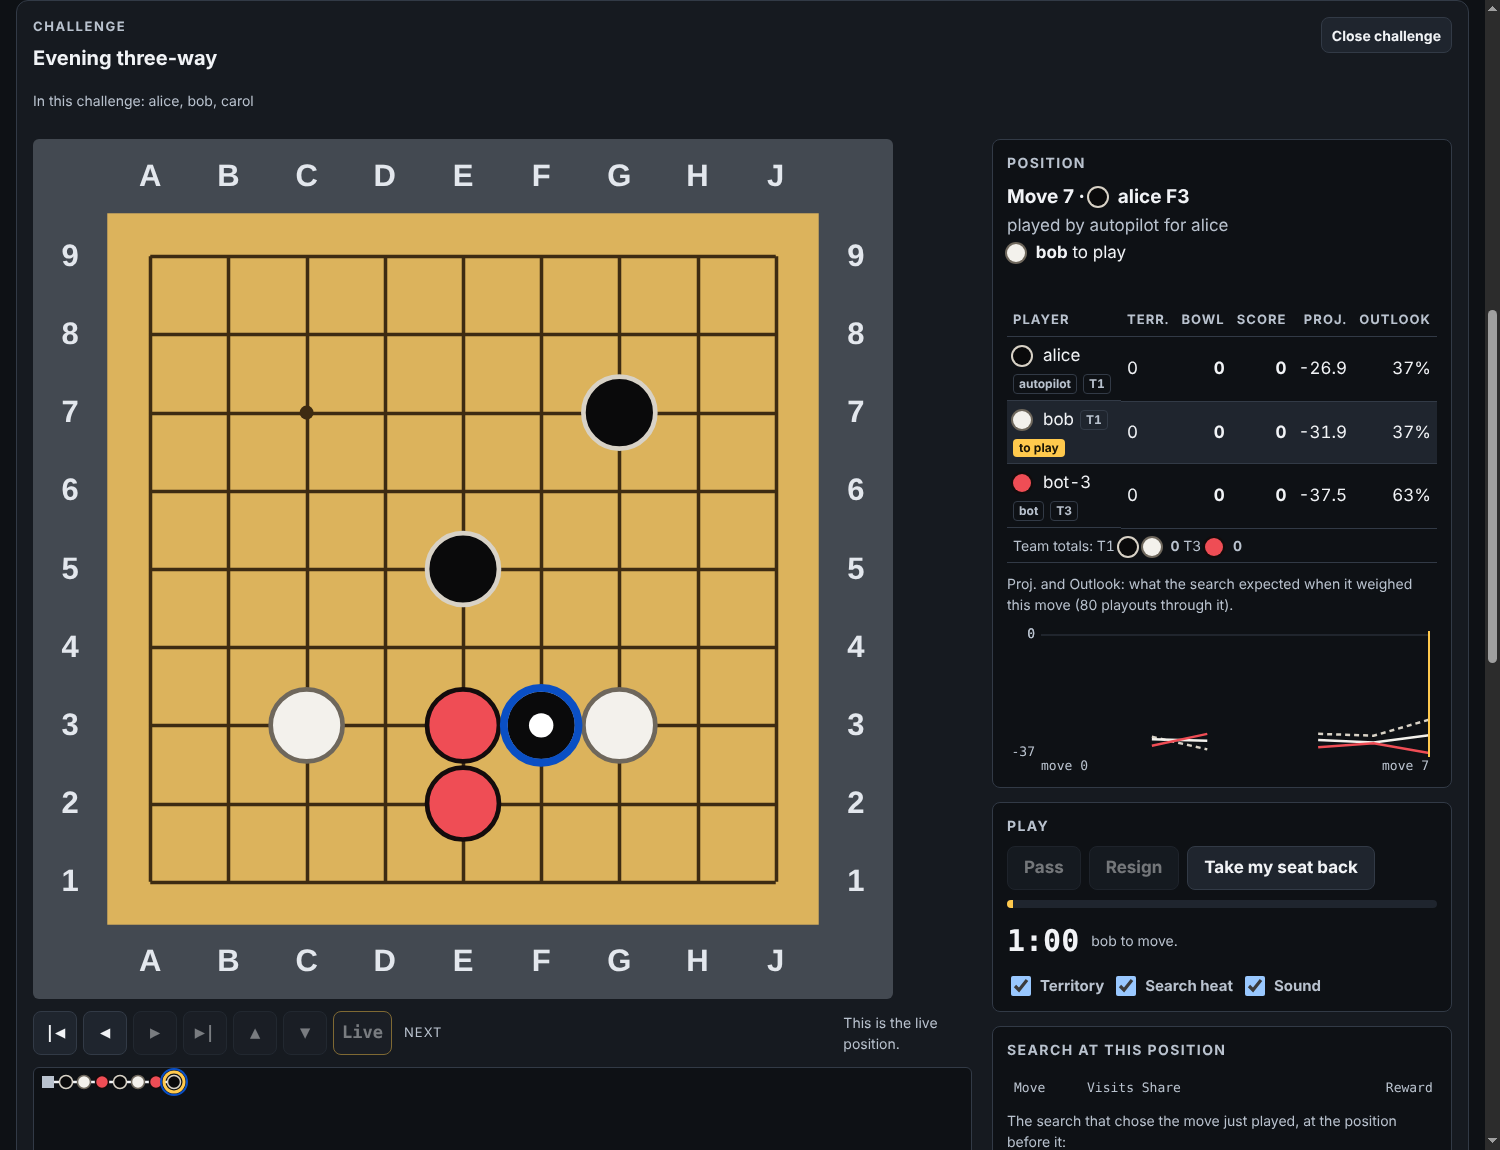
\includegraphics[width=\textwidth]{assets/tour/07-team-and-autopilot.png}
\caption{Playing as a team, on autopilot, seen by alice. Steps: alice: Accept merge; alice: Let a bot play for me.}
\end{figure}
\clearpage

\section{The result}
When every remaining player has passed in a row the game ends. The Chat tab lights up with an unread count; the server announces team scores and the winners in the game conversation. Everyone, players included, can now branch and analyse any position.

\begin{figure}[ht]
\centering
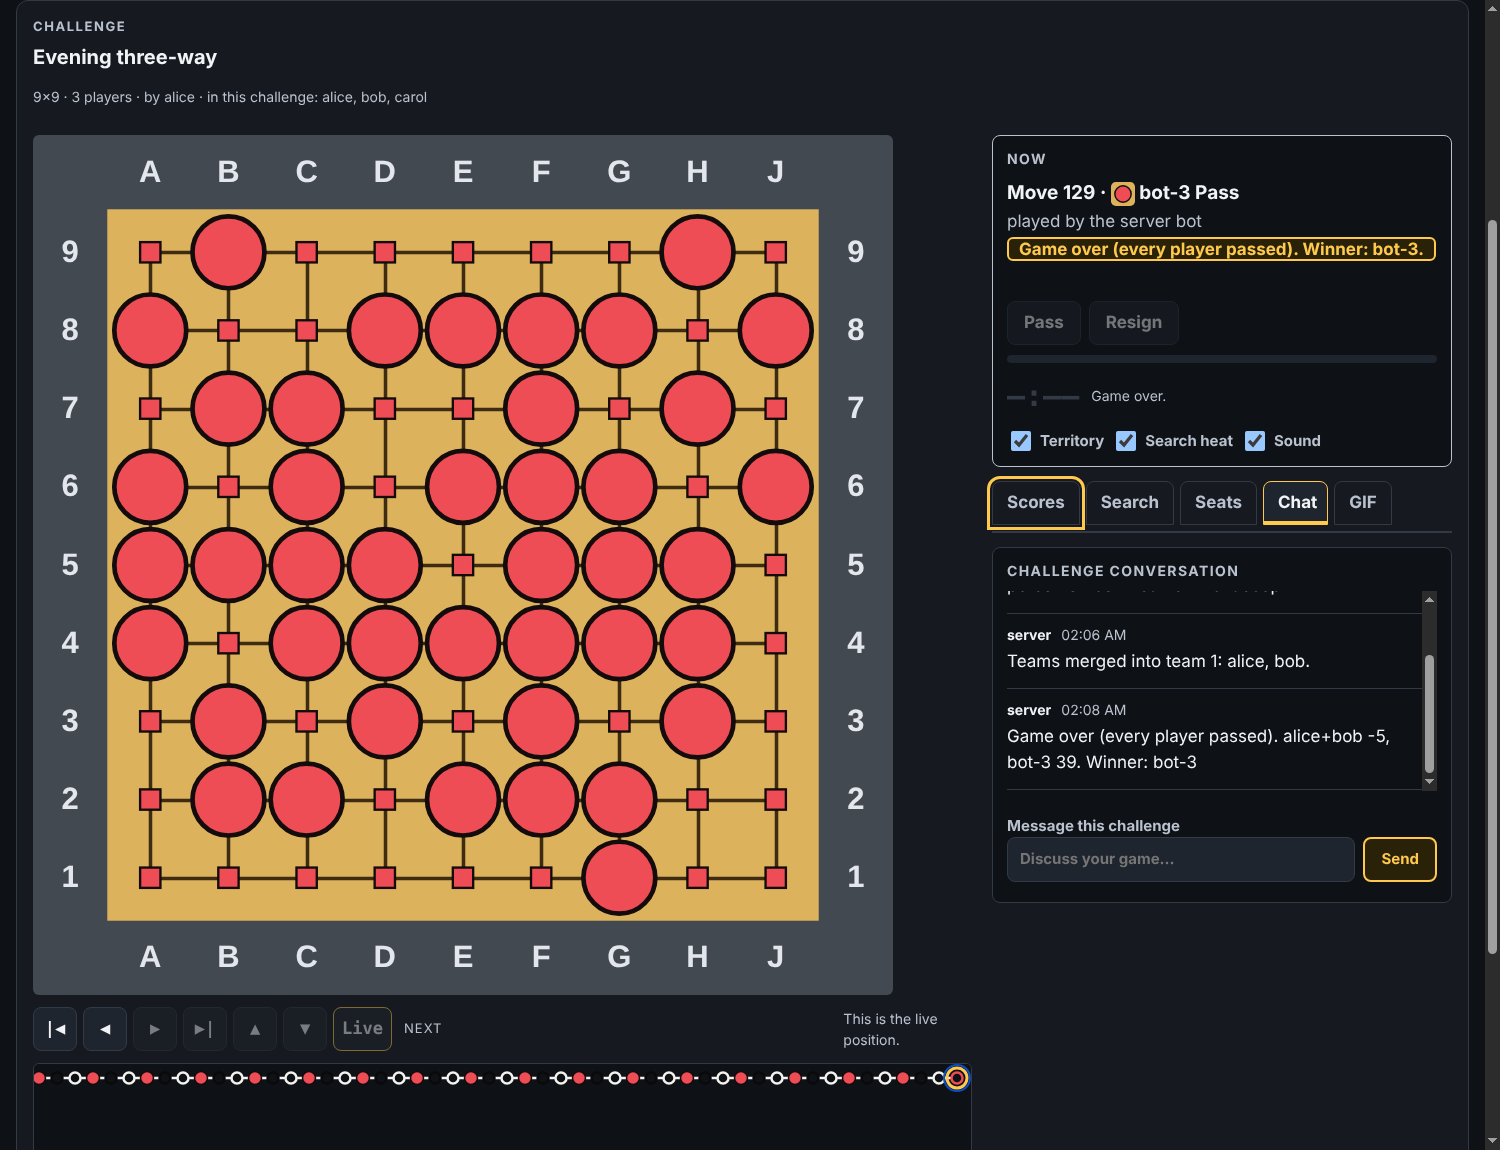
\includegraphics[width=\textwidth]{assets/tour/08-game-over.png}
\caption{The result, seen by alice. Steps: alice passes with the P key, bob with the Pass button, until the bot also passes.}
\end{figure}
\clearpage

\section{Reviewing together}
After the game alice steps back to move 2, passes for the seat to move there and lets the computer pick the next move. Both moves are kept on the server for everyone in the game, and her remark is pinned to the position she was looking at: the Chat tab shows the remarks along the line on the board, so stepping back hides it again and anyone who walks into this variation sees it.

\begin{figure}[ht]
\centering
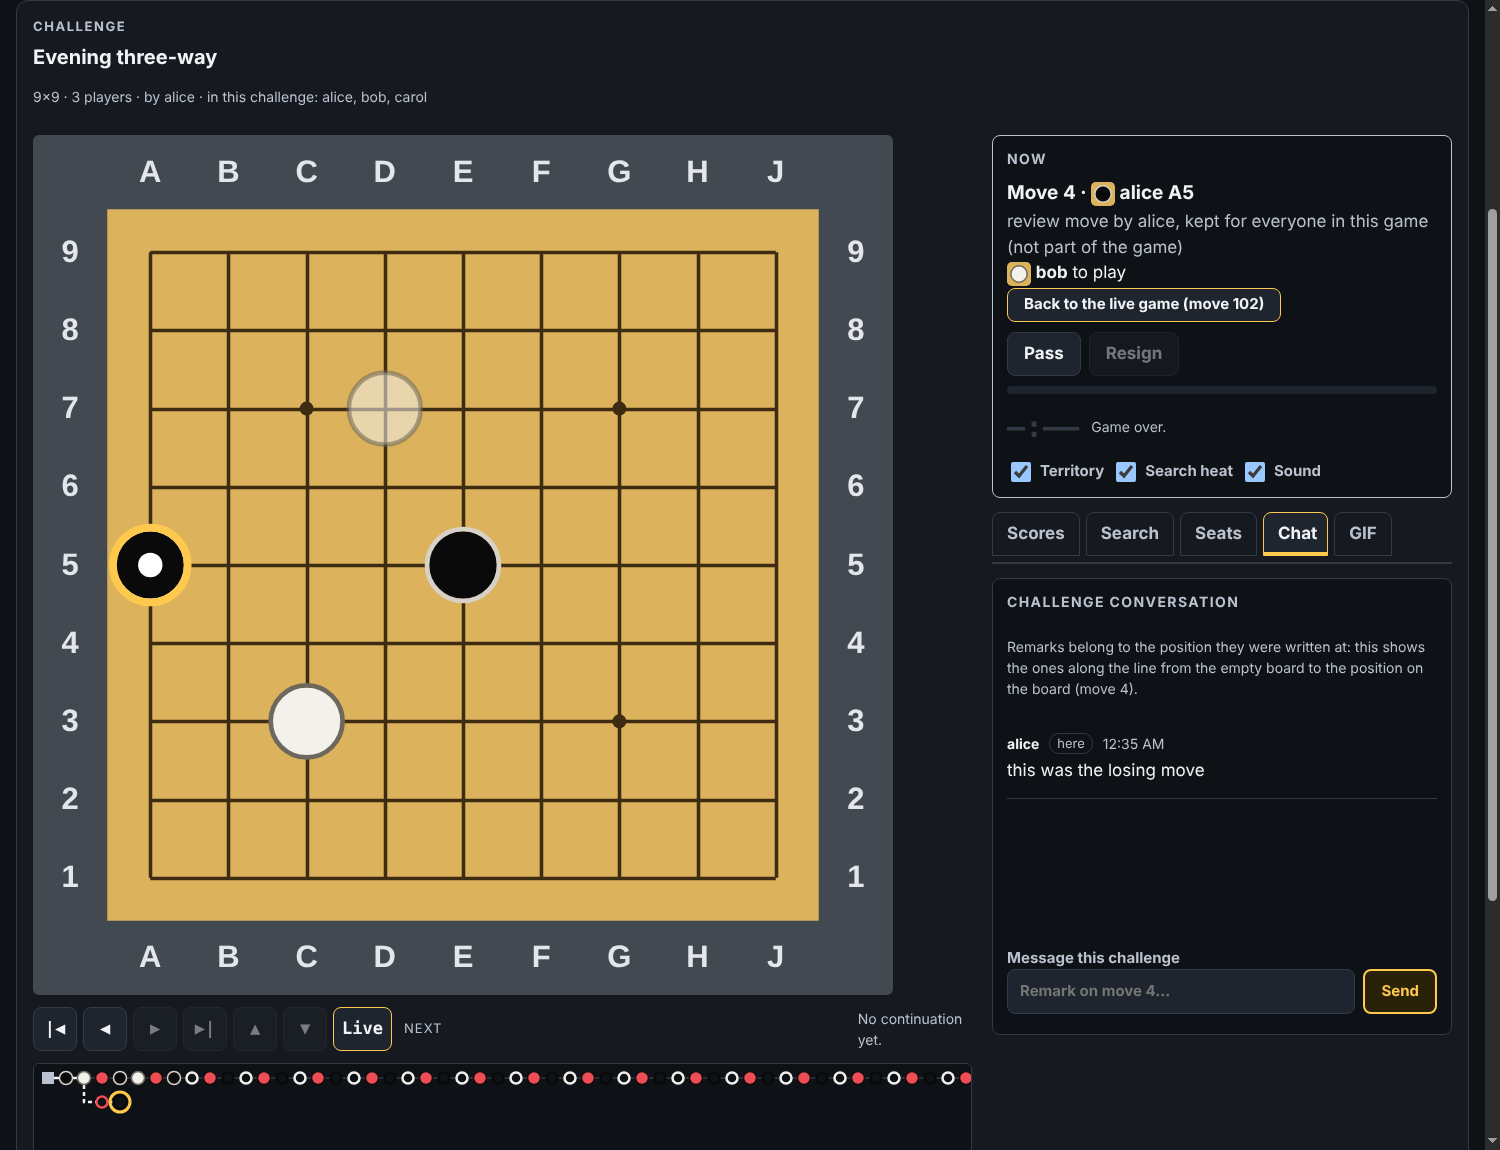
\includegraphics[width=\textwidth]{assets/tour/08a-review-chat.png}
\caption{Reviewing together, seen by alice. Steps: alice: Home, then → twice; alice: P, then C; alice: write a remark in Chat.}
\end{figure}
\clearpage

\section{Rooms and games as tabs}
Every room alice has open is a tab along the top, with + Rooms for finding and creating rooms; inside a room, the Lobby (its conversation and challenge list) comes first and every open game has its own tab. Tabs stay alive in the background: a game keeps its variations and analysis, and a tab shows a badge when a move or a merge waits for her or messages arrive. Responses only ever land in the tab that asked for them.

\begin{figure}[ht]
\centering
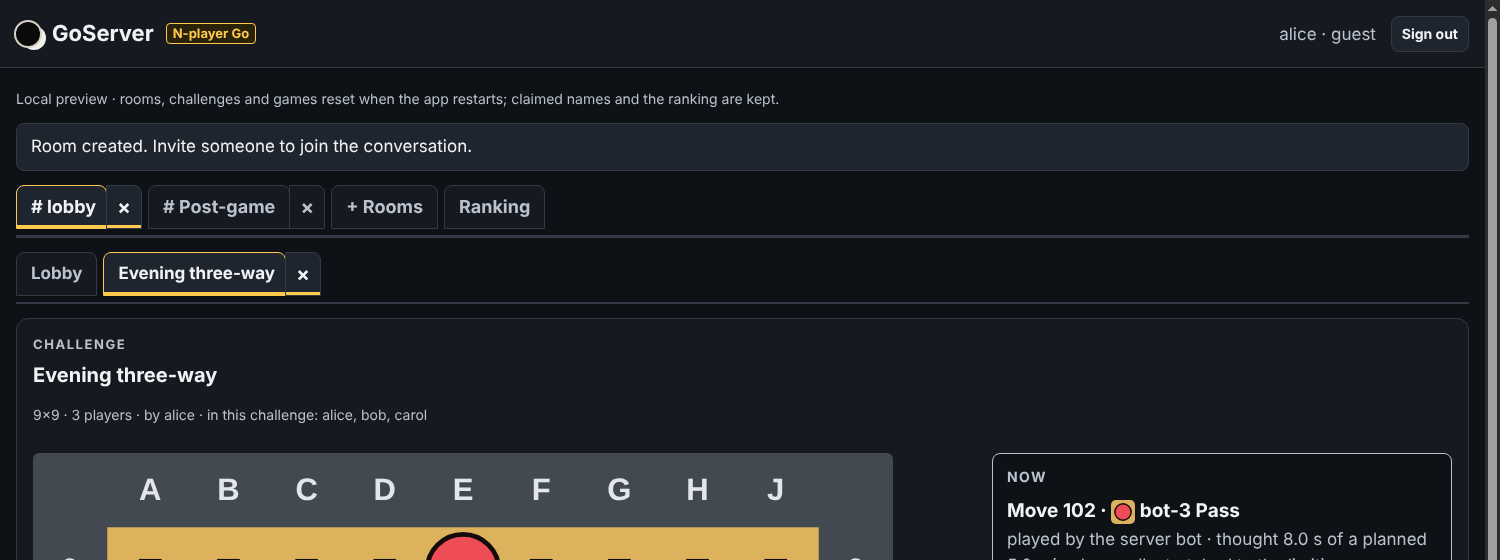
\includegraphics[width=\textwidth]{assets/tour/09-tabs.png}
\caption{Rooms and games as tabs, seen by alice. Steps: alice: + Rooms, create Post-game; alice: back to the lobby room tab.}
\end{figure}
\clearpage
}{}

% ---------------------------------------------------------------------------
\chapter{Known gaps}
\label{ch:gaps}
This chapter is the work queue. When an item is closed, remove it here and add
its evidence under \path{reports/}.
\begin{itemize}
  \item Handicaps and tournaments.
  \item Persistence of rooms, games and chat across restarts, and SGF export of
  game records (claims and rated results already persist).
  \item Password change and recovery; names that look alike in other scripts
  (homoglyphs) are not treated as the same name.
  \item Rating uncertainty is not shown; a player with few games simply stays
  near 1500.
  \item Push transport: the browser polls (every 0.5 seconds while playing).
  \item Reconnect grace beyond reloading the page, and moderation.
  \item Accounts: an unclaimed display name is trusted for the life of the
  server; anyone may sign in with a claimed name's password, so the password is
  the account.
  \item Protobuf byte conformance of the JSON harness.
  \item Server-side enforcement of the analysis rule for seated players, which
  is impossible by nature for public positions.
\end{itemize}

\appendix
\IfFileExists{../renders/views.tex}{\input{../renders/views.tex}}{%
  \chapter{Task catalog}\label{ch:catalog}Run \texttt{make views} to generate the task figures.}

\chapter{How the project got here}
The git history is the authoritative log. In outline: the first slice was a
server-only room, challenge and chat service with typed correlation and
replay; working room creation and a real browser followed; then N-player play
with server bots, deadlines and scoring; then parity with the N-Player Go Lab
(seat plans, autopilot, teams and merges, search summaries, history,
variations and local analysis). On November 1, 2026 the project moved to the
repository's current conventions: review in git instead of recorded approval
gates, a project-level Makefile, figures derived from the checked catalog, and
this book rewritten to describe the system as it is.
\end{document}
